\chapter{Bugzilla \\ 
\small{\textit{-- Ivan Farfan, Johan Jaramillo, Ryan Davis}}} 
\index{Bugzilla} \index{Chapter::Bugzilla} \label{Chapter::Bugzilla}
\section{Overview}

For this part of the assignment, Bugzilla, a web-based bug tracking system, was deployed on a DigitalOcean Droplet using Docker containers. Instead of using a prebuilt image with MariaDB included, we configured two separate containers: one running Bugzilla and another running MySQL as the database backend. This approach ensured greater flexibility and easier debugging when dealing with database connection issues.

\noindent
The Bugzilla image used was the official image available on Docker Hub:

\begin{center}
\url{https://hub.docker.com/r/bugzilla/bugzilla-dev}
\end{center}

\section{Configuration Steps}
\subsection{Droplet Setup}
\begin{itemize}
    \item A new DigitalOcean Droplet was created running \texttt{Ubuntu 25.04}.
    \item Docker was installed using the standard package manager:
    \begin{verbatim}
    apt update
    apt install docker.io -y
    \end{verbatim}
    \item Verified that Docker was running correctly with:
    \begin{verbatim}
    systemctl status docker
    \end{verbatim}
\end{itemize}

\subsection{MySQL Container Configuration}
\begin{itemize}
    \item Pulled the MySQL 5.7 image and started the container:
    \begin{verbatim}
    docker run -d \
      --name bugzilla-mysql \
      -e MYSQL_ROOT_PASSWORD=root \
      -e MYSQL_DATABASE=bugs \
      -e MYSQL_USER=bugs \
      -e MYSQL_PASSWORD=bugspass \
      mysql:5.7
    \end{verbatim}
    \item This container served as the database backend for Bugzilla.
    \item Once running, the container could be verified using:
    \begin{verbatim}
    docker ps
    \end{verbatim}
\end{itemize}

\subsection{Bugzilla Container Setup}
\begin{itemize}
    \item Pulled and started the Bugzilla container:
    \begin{verbatim}
    docker run -d \
      --name bugzilla \
      -p 8080:80 \
      --link bugzilla-mysql:mysql \
      bugzilla/bugzilla-dev
    \end{verbatim}
    \item Accessed the Bugzilla container shell:
    \begin{verbatim}
    docker exec -it bugzilla bash
    cd /var/www/html/bugzilla
    \end{verbatim}
    \item Edited the \texttt{localconfig} file to match the MySQL settings:
    \begin{verbatim}
    $db_driver = 'mysql';
    $db_name   = 'bugs';
    $db_user   = 'bugs';
    $db_pass   = 'bugspass';
    $db_host   = 'bugzilla-mysql';
    \end{verbatim}
    \item Ran the initial setup:
    \begin{verbatim}
    ./checksetup.pl
    \end{verbatim}
    \item Created the Bugzilla administrator account when prompted.
\end{itemize}

\subsection{Troubleshooting and Resource Limitations}
During deployment, the initial droplet used was one of the smallest and most affordable DigitalOcean options, which lacked sufficient memory to run both containers simultaneously. This caused the MySQL container to fail with the following error:
\begin{verbatim}
Can't connect to local MySQL server through socket '/var/lib/mysql/mysql.sock'
\end{verbatim}

\noindent
To resolve this issue:
\begin{itemize}
    \item The droplet was temporarily powered off to modify its plan.
    \item It was upgraded to the following configuration:
    \begin{center}
        \begin{tabular}{|l|l|}
        \hline
        Plan Type & Basic Premium Intel \\
        \hline
        vCPUs & 2 \\
        \hline
        Memory & 2 GB \\
        \hline
        Disk & 25 GB \\
        \hline
        Bandwidth & 3 TB \\
        \hline
        Cost & \$24/month (\$0.036/hr) \\
        \hline
        \end{tabular}
    \end{center}
    \item After resizing, both containers were able to start successfully without memory-related errors.
\end{itemize}

\subsection{Apache Restart and Verification}
\begin{itemize}
    \item Restarted Apache within the Bugzilla container:
    \begin{verbatim}
    apachectl restart
    \end{verbatim}
    \item Verified that the Bugzilla web interface was accessible through:
    \begin{center}
    \texttt{http://167.71.179.151:8080/bugzilla/}
    \end{center}
\end{itemize}

\section{Result}
After adjusting the droplet resources and reconfiguring the database settings, Bugzilla successfully initialized and connected to the MySQL backend. The administrator account was created, and the web interface became fully functional and accessible through the public IP and port 8080.

\section{Container Web Access}
To confirm that the Bugzilla instance was properly running and publicly accessible, the container was tested by visiting the droplet’s IP address on port 8080. The Bugzilla login interface loaded successfully, verifying that both the Apache server and MySQL backend were operational.

\begin{figure}[H]
    \centering
    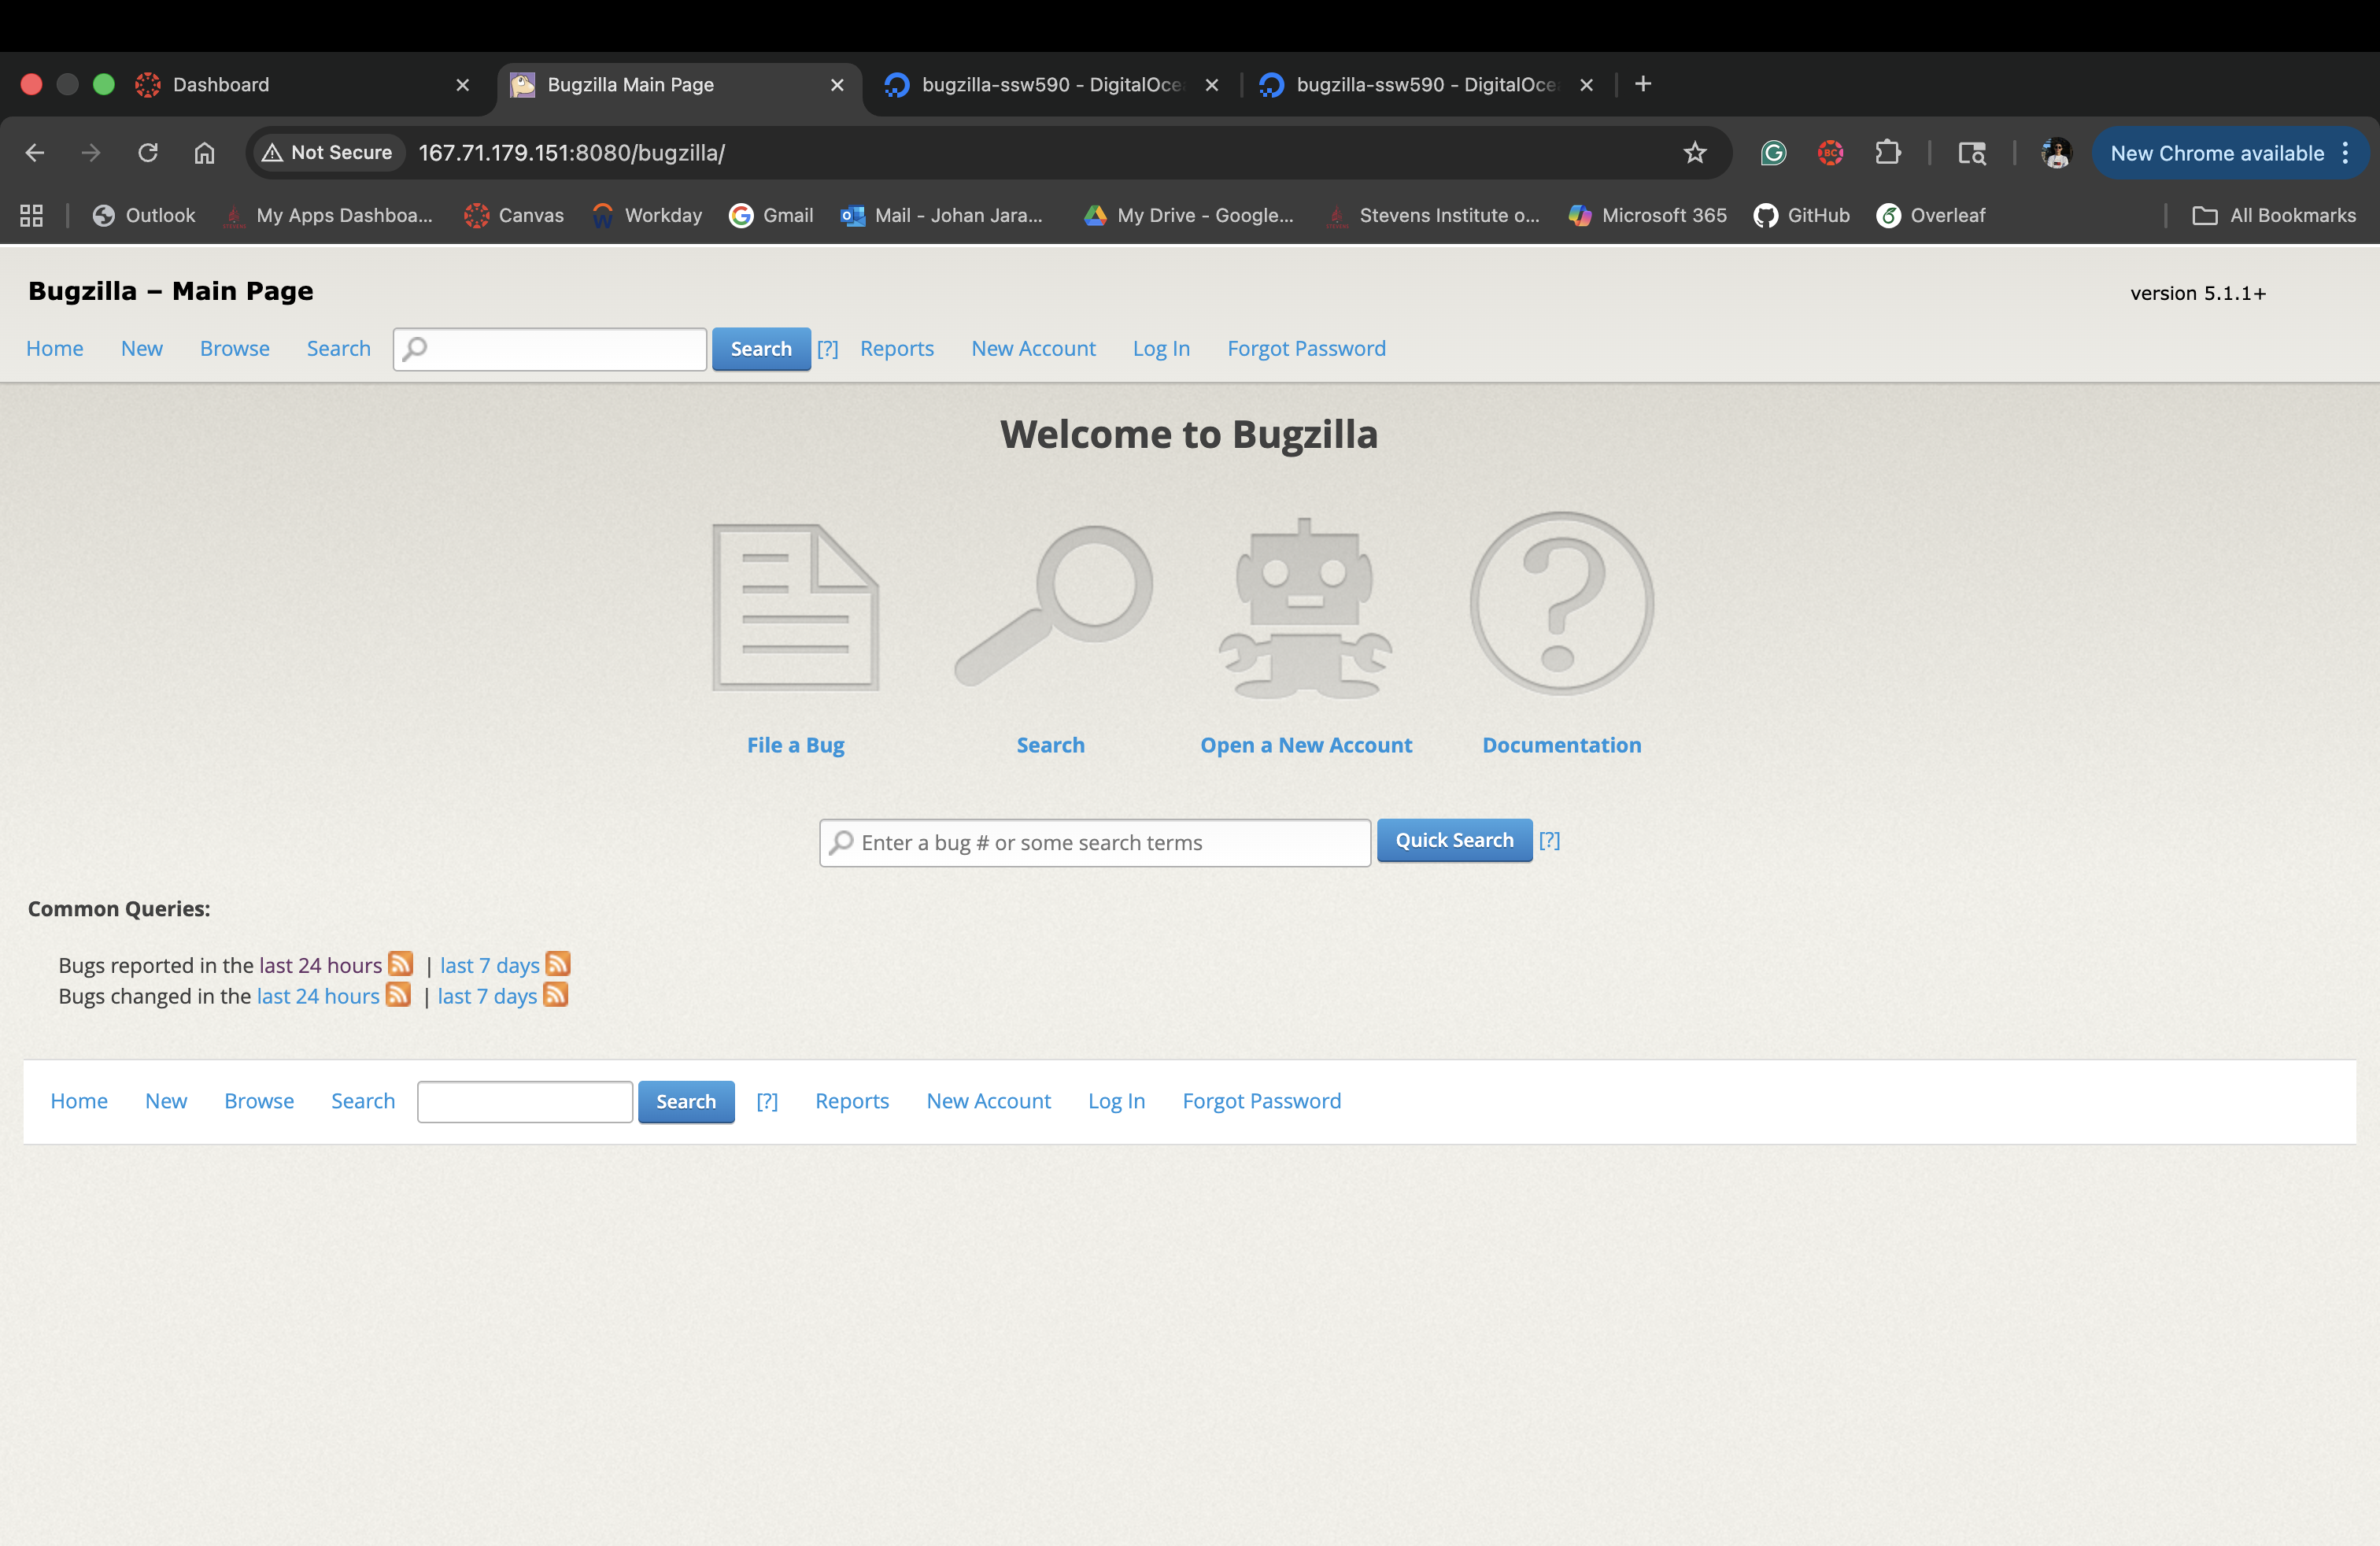
\includegraphics[width=0.9\textwidth]{png/bugzilla.png}
    \caption{Bugzilla web interface confirming successful container deployment on port 8080.}
    \label{fig:bugzilla-port}
\end{figure}
